\documentclass[12pt,letterpaper]{article}
\usepackage{graphicx,textcomp}
\usepackage{natbib}
\usepackage{setspace}
\usepackage{fullpage}
\usepackage{color}
\usepackage[reqno]{amsmath}
\usepackage{amsthm}
\usepackage{fancyvrb}
\usepackage{amssymb,enumerate}
\usepackage[all]{xy}
\usepackage{endnotes}
\usepackage{lscape}
\newtheorem{com}{Comment}
\usepackage{float}
\usepackage{hyperref}
\newtheorem{lem} {Lemma}
\newtheorem{prop}{Proposition}
\newtheorem{thm}{Theorem}
\newtheorem{defn}{Definition}
\newtheorem{cor}{Corollary}
\newtheorem{obs}{Observation}
\usepackage[compact]{titlesec}
\usepackage{dcolumn}
\usepackage{tikz}
\usetikzlibrary{arrows}
\usepackage{multirow}
\usepackage{xcolor}
\newcolumntype{.}{D{.}{.}{-1}}
\newcolumntype{d}[1]{D{.}{.}{#1}}
\definecolor{light-gray}{gray}{0.65}
\usepackage{url}
\usepackage{listings}
\usepackage{color}

\definecolor{codegreen}{rgb}{0,0.6,0}
\definecolor{codegray}{rgb}{0.5,0.5,0.5}
\definecolor{codepurple}{rgb}{0.58,0,0.82}
\definecolor{backcolour}{rgb}{0.95,0.95,0.92}

\lstdefinestyle{mystyle}{
	backgroundcolor=\color{backcolour},   
	commentstyle=\color{codegreen},
	keywordstyle=\color{magenta},
	numberstyle=\tiny\color{codegray},
	stringstyle=\color{codepurple},
	basicstyle=\footnotesize,
	breakatwhitespace=false,         
	breaklines=true,                 
	captionpos=b,                    
	keepspaces=true,                 
	numbers=left,                    
	numbersep=5pt,                  
	showspaces=false,                
	showstringspaces=false,
	showtabs=false,                  
	tabsize=2
}
\lstset{style=mystyle}
\newcommand{\Sref}[1]{Section~\ref{#1}}
\newtheorem{hyp}{Hypothesis}

\title{Problem Set 3 \\
	\large Applied Stats/Quant Methods }
\date{Due: November 16, 2025}
\author{Matilda Tomatis}



\begin{document}
	\maketitle
	\section*{Instructions}
	\begin{itemize}
		\item Please show your work! You may lose points by simply writing in the answer. If the problem requires you to execute commands in \texttt{R}, please include the code you used to get your answers. Please also include the \texttt{.R} file that contains your code. If you are not sure if work needs to be shown for a particular problem, please ask.
	\item Your homework should be submitted electronically on GitHub.
	\item This problem set is due before 23:59 on Thursday November 13, 2025. No late assignments will be accepted.

	\end{itemize}

		\vspace{.25cm}
	
\noindent In this problem set, you will run several regressions and create an add variable plot (see the lecture slides) in \texttt{R} using the \texttt{incumbents\_subset.csv} dataset. Include all of your code.

	\vspace{.5cm}
\section*{Question 1}
\vspace{.25cm}
\noindent We are interested in knowing how the difference in campaign spending between incumbent and challenger affects the incumbent's vote share. 
	\begin{enumerate}
		\item Run a regression where the outcome variable is \texttt{voteshare} and the explanatory variable is \texttt{difflog}.	
		\vspace{0.50cm}
		\item Make a scatterplot of the two variables and add the regression line. 	
		\vspace{0.50cm}
		\item Save the residuals of the model in a separate object.	
		\vspace{0.50cm}
		\item Write the prediction equation.
	\end{enumerate}
	
		\vspace{2cm}
\noindent\textbf{Answer 1.1}\\

\vspace{0.5cm}
\noindent A bivariate linear regression is estimated with vote share (\texttt{voteshare}) as the dependent variable and the difference in log spending (\texttt{difflog}) as the explanatory variable. The estimated coefficient $\beta_1 = 0.042$ implies that, for each one-unit increase in the spending difference between the incumbent and the challenger (in log units), the incumbent’s vote share increases by approximately 0.042.
\lstinputlisting[language=R, firstline=40, lastline=40]{PS03_Tomatis.R} 
\begin{table}[!htbp] \centering 
	\caption{First bivariate regression model} 
	\label{} 
	\begin{tabular}{@{\extracolsep{5pt}}lc} 
		\\[-1.8ex]\hline 
		\hline \\[-1.8ex] 
		& \multicolumn{1}{c}{\textit{Dependent variable:}} \\ 
		\cline{2-2} 
		\\[-1.8ex] & voteshare \\ 
		\hline \\[-1.8ex] 
		difflog & 0.042$^{***}$ \\ 
		& (0.001) \\ 
		& \\ 
		Constant & 0.579$^{***}$ \\ 
		& (0.002) \\ 
		& \\ 
		\hline \\[-1.8ex] 
		Observations & 3,193 \\ 
		R$^{2}$ & 0.367 \\ 
		Adjusted R$^{2}$ & 0.367 \\ 
		Residual Std. Error & 0.079 (df = 3191) \\ 
		F Statistic & 1,852.791$^{***}$ (df = 1; 3191) \\ 
		\hline 
		\hline \\[-1.8ex] 
		\textit{Note:}  & \multicolumn{1}{r}{$^{*}$p$<$0.1; $^{**}$p$<$0.05; $^{***}$p$<$0.01} \\ 
	\end{tabular} 
\end{table} 
\vspace{1cm}

\noindent\textbf{Answer 1.2}\\

\vspace{0.5cm}
\noindent Follows the code to obtain a scatterplot having \texttt{voteshare} on the y-axis and \texttt{difflog} on the x-axis, added is their fitted regression line with its shaded confidence interval.

\lstinputlisting[language=R, firstline=48, lastline=52]{PS03_Tomatis.R} 
\begin{figure}[H]\centering
	\caption{\footnotesize Scatterplot of incumbent vote share against spending difference with fitted regression line}
	\label{fig:q1_scatter}
	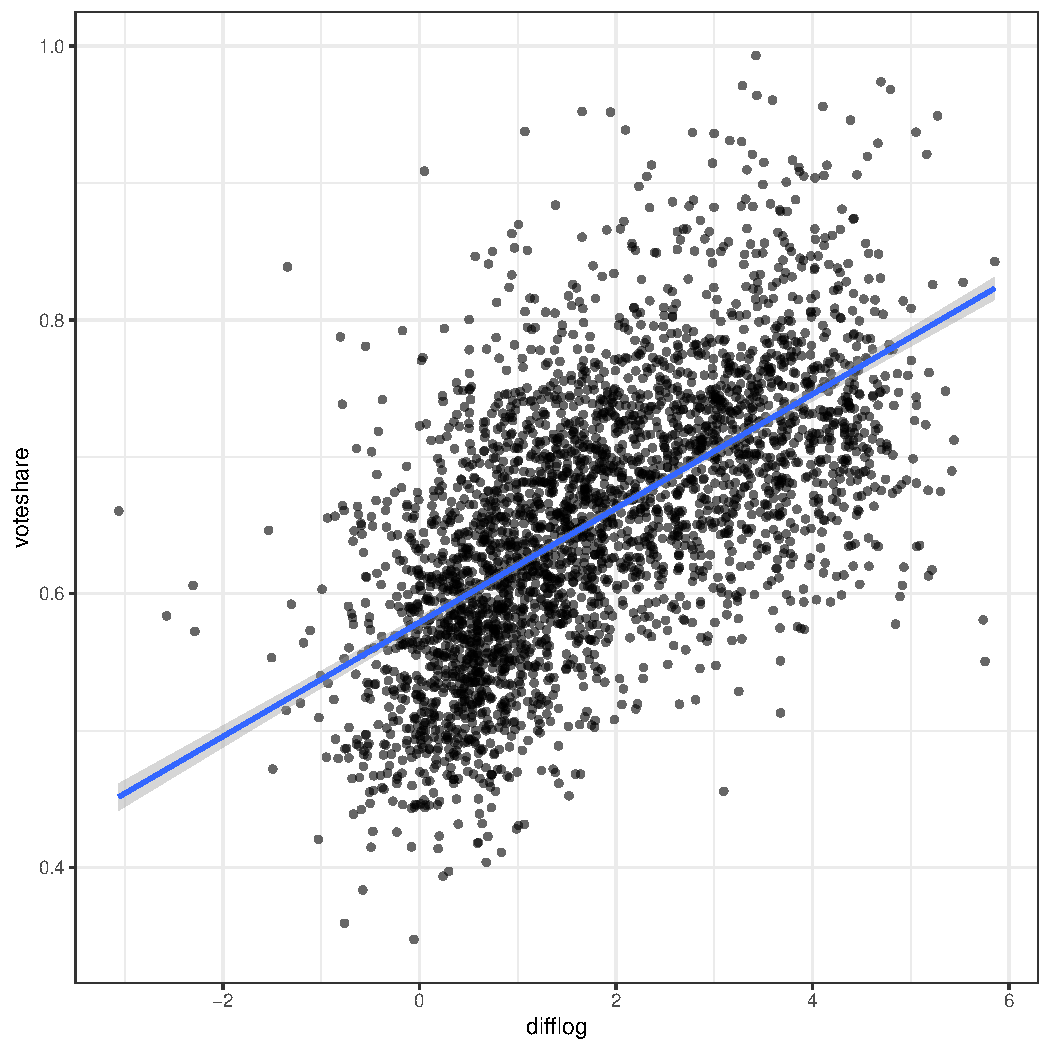
\includegraphics[width=\textwidth]{q1_scatter.pdf}
\end{figure}
\vspace{1cm}
\noindent\textbf{Answer 1.3}\\

\vspace{0.5cm}
\noindent The residuals obtained from regressing \texttt{voteshare} on \texttt{difflog} are stored in a separate object.

\lstinputlisting[language=R, firstline=61, lastline=61]{PS03_Tomatis.R} 

\vspace{1cm}
\noindent\textbf{Answer 1.4}\\

\vspace{0.5cm}
\noindent The prediction equation considers the estimated coefficient to predict unknown \texttt{voteshare} values given an appropriate \texttt{difflog} Xi.
\[
\widehat{\text{voteshare}}_i = \hat{\beta}_0 + \hat{\beta}_1 \, \text{difflog}_i
\]

\vspace{2.5cm}

\section*{Question 2}
\noindent We are interested in knowing how the difference between incumbent and challenger's spending and the vote share of the presidential candidate of the incumbent's party are related.	\vspace{.25cm}
	\begin{enumerate}
		\item Run a regression where the outcome variable is \texttt{presvote} and the explanatory variable is \texttt{difflog}.	
		\vspace{0.5cm}
		\item Make a scatterplot of the two variables and add the regression line. 
		\vspace{0.5cm}
		\item Save the residuals of the model in a separate object.	\vspace{0.5cm}
		\item Write the prediction equation.
	\end{enumerate}
	
	\vspace{2cm}
\noindent\textbf{Answer 2.1}\\

\vspace{0.5cm}
\noindent A bivariate linear regression is estimated with incumbent's party presidential vote share (\texttt{presvote}) as the dependent variable and the difference in log spending (\texttt{difflog}) as the explanatory variable. The estimated coefficient $\beta_1 = 0.023837$ implies that, for each one-unit increase in the spending difference between the incumbent and the challenger (in log units), the presidential candidate of the incumbent’s part is expected to have an increases of approximately 2.4 percentage points.
\lstinputlisting[language=R, firstline=68, lastline=68]{PS03_Tomatis.R} 
\begin{table}[!htbp] \centering 
	\caption{Second bivariate regression model} 
	\label{} 
	\begin{tabular}{@{\extracolsep{5pt}}lc} 
		\\[-1.8ex]\hline 
		\hline \\[-1.8ex] 
		& \multicolumn{1}{c}{\textit{Dependent variable:}} \\ 
		\cline{2-2} 
		\\[-1.8ex] & presvote \\ 
		\hline \\[-1.8ex] 
		difflog & 0.024$^{***}$ \\ 
		& (0.001) \\ 
		& \\ 
		Constant & 0.508$^{***}$ \\ 
		& (0.003) \\ 
		& \\ 
		\hline \\[-1.8ex] 
		Observations & 3,193 \\ 
		R$^{2}$ & 0.088 \\ 
		Adjusted R$^{2}$ & 0.088 \\ 
		Residual Std. Error & 0.110 (df = 3191) \\ 
		F Statistic & 307.715$^{***}$ (df = 1; 3191) \\ 
		\hline 
		\hline \\[-1.8ex] 
		\textit{Note:}  & \multicolumn{1}{r}{$^{*}$p$<$0.1; $^{**}$p$<$0.05; $^{***}$p$<$0.01} \\ 
	\end{tabular} 
\end{table} 
\vspace{1cm}

\noindent\textbf{Answer 2.2}\\

\vspace{0.5cm}
\noindent Repeating the same procedure from before we obtain a new scatterplot, this second time \texttt{presvote} lays on the y-axis and the regression line is obtained by regressing it on \texttt{difflog}.

\lstinputlisting[language=R, firstline=76, lastline=80]{PS03_Tomatis.R} 
\begin{figure}[H]\centering
	\caption{\footnotesize Scatterplot of incumbent's party presidential candidate's vote share against spending difference, with fitted regression line}
	\label{fig:q2_scatter}
	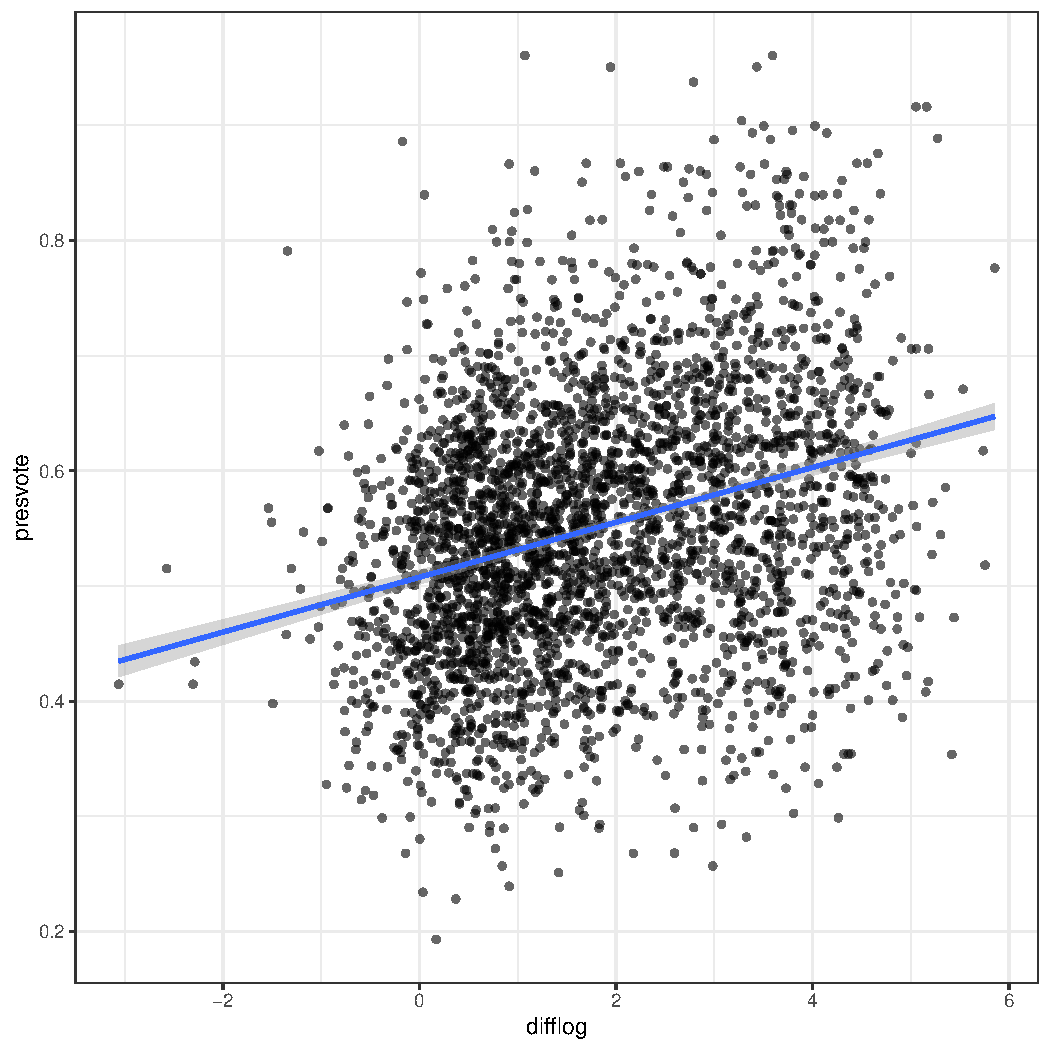
\includegraphics[width=\textwidth]{q2_scatter.pdf}
\end{figure}
\vspace{1cm}
\noindent\textbf{Answer 2.3}\\

\vspace{0.5cm}
\noindent The residuals obtained from the second simple linear regression are stored in a separate object.

\lstinputlisting[language=R, firstline=89, lastline=89]{PS03_Tomatis.R} 

\vspace{1cm}
\noindent\textbf{Answer 2.4}\\

\vspace{0.5cm}
\noindent The prediction equation considers the estimated coefficient to predict unknown \texttt{presvote} values given an appropriate \texttt{difflog} Xi.
\[
\widehat{\text{presvote}}_i = \hat{\beta}_0 + \hat{\beta}_1 \, \text{difflog}_i
\]

\vspace{2.5cm}

\section*{Question 3}

\noindent We are interested in knowing how the vote share of the presidential candidate of the incumbent's party is associated with the incumbent's electoral success.
	\vspace{.25cm}
	\begin{enumerate}
		\item Run a regression where the outcome variable is \texttt{voteshare} and the explanatory variable is \texttt{presvote}.
			\vspace{0.5cm}
		\item Make a scatterplot of the two variables and add the regression line. 
			\vspace{0.5cm}
		\item Write the prediction equation.
	\end{enumerate}
	
	\vspace{2cm}
\noindent\textbf{Answer 3.1}\\

\vspace{0.5cm}
\noindent For the last estimation of the $\beta_1$ and $\beta_0$ coefficients using data from the \textbf{incumbent\_subset} dataset, a bivariate regression with \texttt{voteshare} as the dependent variable and \texttt{presvote} as the explanatory one. The estimated coefficient $\hat{\beta}_1 = 0.388$ suggests that, on average, when the incumbent party’s presidential candidate performs better by one unit in vote share, the incumbent’s own vote share increases by approximately 0.388 units
\lstinputlisting[language=R, firstline=95, lastline=95]{PS03_Tomatis.R} 
\begin{table}[!htbp] \centering 
	\caption{Third bivariate regression model} 
	\label{} 
	\begin{tabular}{@{\extracolsep{5pt}}lc} 
		\\[-1.8ex]\hline 
		\hline \\[-1.8ex] 
		& \multicolumn{1}{c}{\textit{Dependent variable:}} \\ 
		\cline{2-2} 
		\\[-1.8ex] & voteshare \\ 
		\hline \\[-1.8ex] 
		presvote & 0.388$^{***}$ \\ 
		& (0.013) \\ 
		& \\ 
		Constant & 0.441$^{***}$ \\ 
		& (0.008) \\ 
		& \\ 
		\hline \\[-1.8ex] 
		Observations & 3,193 \\ 
		R$^{2}$ & 0.206 \\ 
		Adjusted R$^{2}$ & 0.206 \\ 
		Residual Std. Error & 0.088 (df = 3191) \\ 
		F Statistic & 826.950$^{***}$ (df = 1; 3191) \\ 
		\hline 
		\hline \\[-1.8ex] 
		\textit{Note:}  & \multicolumn{1}{r}{$^{*}$p$<$0.1; $^{**}$p$<$0.05; $^{***}$p$<$0.01} \\ 
	\end{tabular} 
\end{table}
\vspace{1cm}

\noindent\textbf{Answer 3.2}\\

\vspace{0.5cm}
\noindent Once again, suing the same methods, a scatterplot of our two variables of interest is made and their simple linear regression line is added.

\lstinputlisting[language=R, firstline=103, lastline=106]{PS03_Tomatis.R} 
\begin{figure}[H]\centering
	\caption{\footnotesize Scatterplot of incumbent's party overall vote share against incumbent's party presidential candidate's vote share, with fitted regression line}
	\label{fig:q3_scatter}
	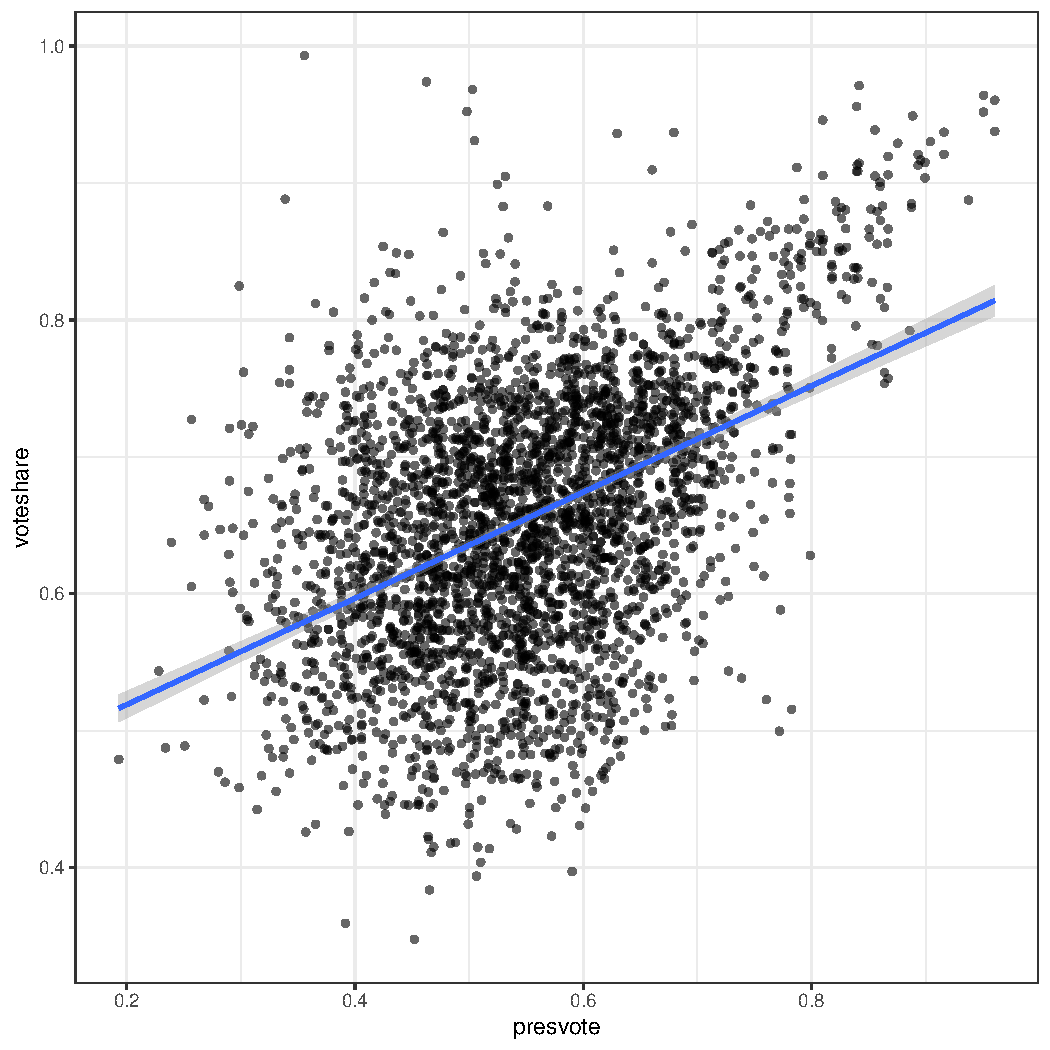
\includegraphics[width=\textwidth]{q3_scatter.pdf}
\end{figure}

\vspace{1cm}
\noindent\textbf{Answer 3.3}\\

\vspace{0.5cm}
\noindent It's presented is the prediction equation for new incumbent's party vote share given a incumbent's party presidential candidate's vote share.
\[
\widehat{\text{voteshare}}_i = \hat{\beta}_0 + \hat{\beta}_1 \, \text{presvote}_i
\]

\vspace{2.5cm}
\section*{Question 4}
\noindent The residuals from part (a) tell us how much of the variation in \texttt{voteshare} is $not$ explained by the difference in spending between incumbent and challenger. The residuals in part (b) tell us how much of the variation in \texttt{presvote} is $not$ explained by the difference in spending between incumbent and challenger in the district.
	\begin{enumerate}
		\item Run a regression where the outcome variable is the residuals from Question 1 and the explanatory variable is the residuals from Question 2.	\vspace{6cm}
		\item Make a scatterplot of the two residuals and add the regression line. 	\vspace{6cm}
		\item Write the prediction equation.
	\end{enumerate}
	
	\newpage	

\section*{Question 5}
\noindent What if the incumbent's vote share is affected by both the president's popularity and the difference in spending between incumbent and challenger? 
	\begin{enumerate}
		\item Run a regression where the outcome variable is the incumbent's \texttt{voteshare} and the explanatory variables are \texttt{difflog} and \texttt{presvote}.	\vspace{5cm}
		\item Write the prediction equation.	\vspace{5cm}
		\item What is it in this output that is identical to the output in Question 4? Why do you think this is the case?
	\end{enumerate}




\end{document}
